\lesson{Reactions of Alkanes, Alkenes, and Alkynes}
\subsection{Reaction of Alkanes}
\begin{bulleted-list}
    \item Alkanes are less reactive than alkenes and alkynes
    \item Due to the saturated nature of alkanes, \textbf{substitution reactions}
        \footnote{
            \textbf{Substitution reactions:} Hydrogen atoms can be replaced by halogen atoms, one
            at a time, when an alkane reacts with $\ch{F2}$, $\ch{Cl2}$, or $\ch{Br2}$ in the
            prescence of UV light. Additional substitutions can occur if more halogen molecules
            are present.
        }
        are most common
    \item Halogen atoms can replace hydrogen atoms on the compound
\end{bulleted-list}

\subsection{Elimination Reactions to Produce Alkenes}
In basic conditions (denoted by the $\ch{OH^-}$), a halide ion and hydrogen atom are eliminated from
adjacent carbons, also producing water
\begin{figure}[ht!]
    \centering
    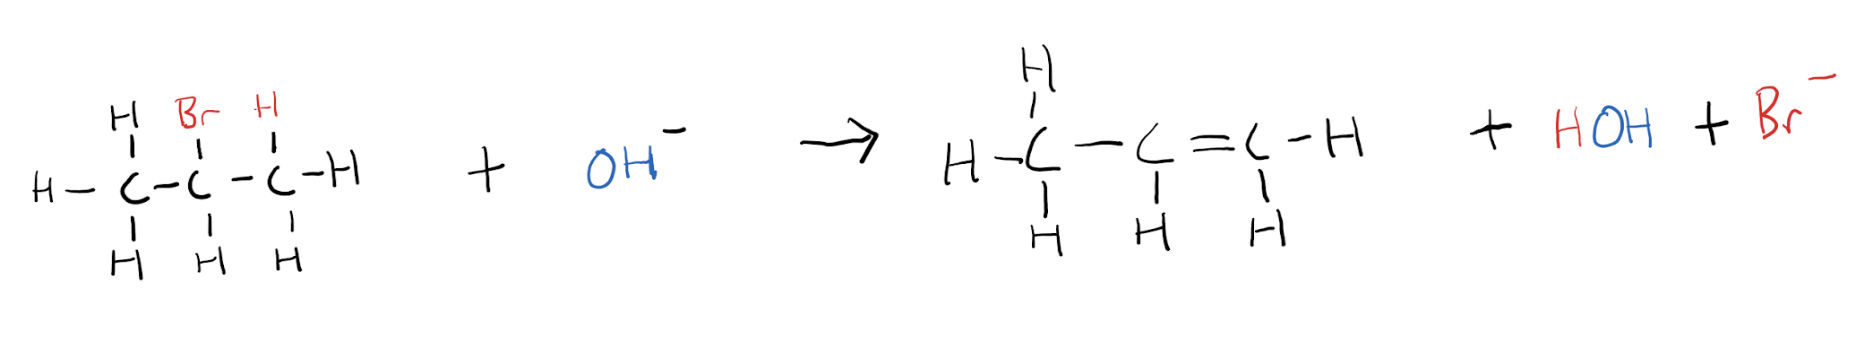
\includegraphics[width=0.8 \textwidth]{../figures/elimination-alkene.png}
\end{figure}

\begin{important}
    Generally, alkenes and alkynes are more reactive than alkanes. Alkenes and alkynes are
    unsaturated; therefore, they can accomodate additional atoms when the triple and/or double
    bonds break-these types of reactions are called \textbf{addition} reactions.
\end{important}

\subsection{Addition Reactions - Hydrogenation}

